% Options for packages loaded elsewhere
\PassOptionsToPackage{unicode}{hyperref}
\PassOptionsToPackage{hyphens}{url}
\PassOptionsToPackage{dvipsnames,svgnames,x11names}{xcolor}
%
\documentclass[
  letterpaper,
  DIV=11,
  numbers=noendperiod,
  oneside]{scrartcl}

\usepackage{amsmath,amssymb}
\usepackage{iftex}
\ifPDFTeX
  \usepackage[T1]{fontenc}
  \usepackage[utf8]{inputenc}
  \usepackage{textcomp} % provide euro and other symbols
\else % if luatex or xetex
  \usepackage{unicode-math}
  \defaultfontfeatures{Scale=MatchLowercase}
  \defaultfontfeatures[\rmfamily]{Ligatures=TeX,Scale=1}
\fi
\usepackage{lmodern}
\ifPDFTeX\else  
    % xetex/luatex font selection
\fi
% Use upquote if available, for straight quotes in verbatim environments
\IfFileExists{upquote.sty}{\usepackage{upquote}}{}
\IfFileExists{microtype.sty}{% use microtype if available
  \usepackage[]{microtype}
  \UseMicrotypeSet[protrusion]{basicmath} % disable protrusion for tt fonts
}{}
\makeatletter
\@ifundefined{KOMAClassName}{% if non-KOMA class
  \IfFileExists{parskip.sty}{%
    \usepackage{parskip}
  }{% else
    \setlength{\parindent}{0pt}
    \setlength{\parskip}{6pt plus 2pt minus 1pt}}
}{% if KOMA class
  \KOMAoptions{parskip=half}}
\makeatother
\usepackage{xcolor}
\usepackage[left=1in,marginparwidth=2.0666666666667in,textwidth=4.1333333333333in,marginparsep=0.3in]{geometry}
\setlength{\emergencystretch}{3em} % prevent overfull lines
\setcounter{secnumdepth}{5}
% Make \paragraph and \subparagraph free-standing
\ifx\paragraph\undefined\else
  \let\oldparagraph\paragraph
  \renewcommand{\paragraph}[1]{\oldparagraph{#1}\mbox{}}
\fi
\ifx\subparagraph\undefined\else
  \let\oldsubparagraph\subparagraph
  \renewcommand{\subparagraph}[1]{\oldsubparagraph{#1}\mbox{}}
\fi


\providecommand{\tightlist}{%
  \setlength{\itemsep}{0pt}\setlength{\parskip}{0pt}}\usepackage{longtable,booktabs,array}
\usepackage{calc} % for calculating minipage widths
% Correct order of tables after \paragraph or \subparagraph
\usepackage{etoolbox}
\makeatletter
\patchcmd\longtable{\par}{\if@noskipsec\mbox{}\fi\par}{}{}
\makeatother
% Allow footnotes in longtable head/foot
\IfFileExists{footnotehyper.sty}{\usepackage{footnotehyper}}{\usepackage{footnote}}
\makesavenoteenv{longtable}
\usepackage{graphicx}
\makeatletter
\def\maxwidth{\ifdim\Gin@nat@width>\linewidth\linewidth\else\Gin@nat@width\fi}
\def\maxheight{\ifdim\Gin@nat@height>\textheight\textheight\else\Gin@nat@height\fi}
\makeatother
% Scale images if necessary, so that they will not overflow the page
% margins by default, and it is still possible to overwrite the defaults
% using explicit options in \includegraphics[width, height, ...]{}
\setkeys{Gin}{width=\maxwidth,height=\maxheight,keepaspectratio}
% Set default figure placement to htbp
\makeatletter
\def\fps@figure{htbp}
\makeatother
% definitions for citeproc citations
\NewDocumentCommand\citeproctext{}{}
\NewDocumentCommand\citeproc{mm}{%
  \begingroup\def\citeproctext{#2}\cite{#1}\endgroup}
\makeatletter
 % allow citations to break across lines
 \let\@cite@ofmt\@firstofone
 % avoid brackets around text for \cite:
 \def\@biblabel#1{}
 \def\@cite#1#2{{#1\if@tempswa , #2\fi}}
\makeatother
\newlength{\cslhangindent}
\setlength{\cslhangindent}{1.5em}
\newlength{\csllabelwidth}
\setlength{\csllabelwidth}{3em}
\newenvironment{CSLReferences}[2] % #1 hanging-indent, #2 entry-spacing
 {\begin{list}{}{%
  \setlength{\itemindent}{0pt}
  \setlength{\leftmargin}{0pt}
  \setlength{\parsep}{0pt}
  % turn on hanging indent if param 1 is 1
  \ifodd #1
   \setlength{\leftmargin}{\cslhangindent}
   \setlength{\itemindent}{-1\cslhangindent}
  \fi
  % set entry spacing
  \setlength{\itemsep}{#2\baselineskip}}}
 {\end{list}}
\usepackage{calc}
\newcommand{\CSLBlock}[1]{\hfill\break#1\hfill\break}
\newcommand{\CSLLeftMargin}[1]{\parbox[t]{\csllabelwidth}{\strut#1\strut}}
\newcommand{\CSLRightInline}[1]{\parbox[t]{\linewidth - \csllabelwidth}{\strut#1\strut}}
\newcommand{\CSLIndent}[1]{\hspace{\cslhangindent}#1}

\usepackage{booktabs}
\usepackage{hyperref}
\usepackage{multirow}
\usepackage{lscape}
\usepackage{changepage}
\usepackage{float}
\floatplacement{figure}{H}
\floatplacement{table}{H}
\KOMAoption{captions}{tableheading}
\makeatletter
\@ifpackageloaded{caption}{}{\usepackage{caption}}
\AtBeginDocument{%
\ifdefined\contentsname
  \renewcommand*\contentsname{Table of contents}
\else
  \newcommand\contentsname{Table of contents}
\fi
\ifdefined\listfigurename
  \renewcommand*\listfigurename{List of Figures}
\else
  \newcommand\listfigurename{List of Figures}
\fi
\ifdefined\listtablename
  \renewcommand*\listtablename{List of Tables}
\else
  \newcommand\listtablename{List of Tables}
\fi
\ifdefined\figurename
  \renewcommand*\figurename{Figure}
\else
  \newcommand\figurename{Figure}
\fi
\ifdefined\tablename
  \renewcommand*\tablename{Table}
\else
  \newcommand\tablename{Table}
\fi
}
\@ifpackageloaded{float}{}{\usepackage{float}}
\floatstyle{ruled}
\@ifundefined{c@chapter}{\newfloat{codelisting}{h}{lop}}{\newfloat{codelisting}{h}{lop}[chapter]}
\floatname{codelisting}{Listing}
\newcommand*\listoflistings{\listof{codelisting}{List of Listings}}
\makeatother
\makeatletter
\makeatother
\makeatletter
\@ifpackageloaded{caption}{}{\usepackage{caption}}
\@ifpackageloaded{subcaption}{}{\usepackage{subcaption}}
\makeatother
\makeatletter
\@ifpackageloaded{sidenotes}{}{\usepackage{sidenotes}}
\@ifpackageloaded{marginnote}{}{\usepackage{marginnote}}
\makeatother
\ifLuaTeX
  \usepackage{selnolig}  % disable illegal ligatures
\fi
\IfFileExists{bookmark.sty}{\usepackage{bookmark}}{\usepackage{hyperref}}
\IfFileExists{xurl.sty}{\usepackage{xurl}}{} % add URL line breaks if available
\urlstyle{same} % disable monospaced font for URLs
\hypersetup{
  pdftitle={HTW},
  pdfauthor={Thomas Gorman; Rob Goldstone},
  pdfkeywords={Learning Generalization, Function Learning, Visuomotor
learning, Training Variability},
  colorlinks=true,
  linkcolor={blue},
  filecolor={Maroon},
  citecolor={Blue},
  urlcolor={Blue},
  pdfcreator={LaTeX via pandoc}}

\title{HTW}
\author{Thomas Gorman \and Rob Goldstone}
\date{2023-10-12}

\begin{document}
\maketitle
\begin{abstract}
In project 1, we applied model-based techniques to quantify and control
for the similarity between training and testing experience, which in
turn enabled us to account for the difference between varied and
constant training via an extended version of a similarity based
generalization model. In project 2, we will go a step further,
implementing a full process model capable of both 1) producing novel
responses and 2) modeling behavior in both the learning and testing
stages of the experiment. Project 2 also places a greater emphasis on
extrapolation performance following training - as varied training has
often been purported to be particularly beneficial in such situations.
\end{abstract}
\renewcommand*\contentsname{Table of contents}
{
\hypersetup{linkcolor=}
\setcounter{tocdepth}{3}
\tableofcontents
}
\section{Introduction}\label{introduction}

In project 1, we applied model-based techniques to quantify and control
for the similarity between training and testing experience, which in
turn enabled us to account for the difference between varied and
constant training via an extended version of a similarity based
generalization model. In project 2, we will go a step further,
implementing a full process model capable of both 1) producing novel
responses and 2) modeling behavior in both the learning and testing
stages of the experiment. Project 2 also places a greater emphasis on
extrapolation performance following training - as varied training has
often been purported to be particularly beneficial in such situations.
Extrapolation has long been a focus of the literature on function
learning (\citeproc{ref-brehmerHypothesesRelationsScaled1974}{Brehmer,
1974}; \citeproc{ref-carrollFunctionalLearningLearning1963}{Carroll,
1963}). Central questions of the function learning literature have
included the relative difficulties of learning various functional forms
(e.g.~linear vs.bilinear vs.~quadratic), and the relative effectiveness
of rule-based vs.~association-based exemplar models vs.~various hybrid
models (\citeproc{ref-bottNonmonotonicExtrapolationFunction2004}{Bott \&
Heit, 2004}; \citeproc{ref-deloshExtrapolationSineQua1997}{DeLosh et
al., 1997}; \citeproc{ref-jonesActiveFunctionLearning2018}{Jones et al.,
2018}; \citeproc{ref-kalishPopulationLinearExperts2004}{Kalish et al.,
2004}; \citeproc{ref-mcdanielPredictingTransferPerformance2009}{M.
Mcdaniel et al., 2009};
\citeproc{ref-mcdanielConceptualBasisFunction2005}{M. A. Mcdaniel \&
Busemeyer, 2005}). However the issue of training variation has received
surprisingly little attention in this area.

\section{Methods}\label{methods}

\subsection{Participants}\label{participants}

Data was collected from 647 participants (after exclusions). The results
shown below consider data from subjects in our initial experiment, which
consisted of 196 participants (106 constant, 90 varied). The follow-up
experiments entailed minor manipulations: 1) reversing the velocity
bands that were trained on vs.~novel during testing; 2) providing
ordinal rather than numerical feedback during training (e.g.~correct,
too low, too high). The data from these subsequent experiments are
largely consistently with our initial results shown below.

\subsection{Task}\label{task}

We developed a novel visuomotor extrapolation task, termed the Hit The
Wall task, wherein participants learned to launch a projectile such that
it hit a rectangle at the far end of the screen with an appropriate
amount of force. Although the projectile had both x and y velocity
components, only the x-dimension was relevant for the task.~
\href{https://pcl.sitehost.iu.edu/tg/HTW/HTW_Index.html?sonaid=}{Link to
task demo}

\subsection{Procedure}\label{procedure}

Upon arrival at the laboratory, participants were provided with a
description of the experiment and signed informed consent forms. They
were then seated in front of a computer equipped with a mouse and were
given instructions on how to perform the ``Hit The Wall'' (HTW)
visuomotor extrapolation task.

The HTW task involved launching projectiles to hit a target displayed on
the computer screen. Participants completed a total of 90 trials during
the training stage. In the varied training condition, participants
encountered three velocity bands (800-1000, 1000-1200, and 1200-1400).
In contrast, participants in the constant training condition encountered
only one velocity band (800-1000).

During the training stage, participants in both conditions also
completed ``no feedback'' trials, where they received no information
about their performance. These trials were randomly interleaved with the
regular training trials.

Following the training stage, participants proceeded to the testing
stage, which consisted of three phases. In the first phase, participants
completed ``no-feedback'' testing from three novel extrapolation bands
(100-300, 350-550, and 600-800), with each band consisting of 15 trials.

In the second phase of testing, participants completed ``no-feedback''
testing from the three velocity bands used during the training stage
(800-1000, 1000-1200, and 1200-1400). In the constant training
condition, two of these bands were novel, while in the varied training
condition, all three bands were encountered during training.

The third and final phase of testing involved ``feedback'' testing for
each of the three extrapolation bands (100-300, 350-550, and 600-800),
with each band consisting of 10 trials. Participants received feedback
on their performance during this phase.

Throughout the experiment, participants' performance was measured by
calculating the distance between the produced x-velocity of the
projectiles and the closest edge of the current velocity band. Lower
distances indicated better performance.

After completing the experiment, participants were debriefed and
provided with an opportunity to ask questions about the study.

\begin{figure*}

\centering{

\includegraphics[width=6in,height=2.5in]{manuscript_files/figure-latex/dot-figure-1.png}

}

\caption{\label{fig-design-e1}Experiment 1 Design. Constant and Varied
participants complete different training conditions.}

\end{figure*}%

\subsection{Analyses Strategy}\label{analyses-strategy}

All data processing and statistical analyses were performed in R version
4.31 Team
(\citeproc{ref-rcoreteamLanguageEnvironmentStatistical2020}{2020}). To
assess differences between groups, we used Bayesian Mixed Effects
Regression. Model fitting was performed with the brms package in R
Bürkner (\citeproc{ref-burknerBrmsPackageBayesian2017}{2017}), and
descriptive stats and tables were extracted with the BayestestR package
Makowski et al.
(\citeproc{ref-makowskiBayestestRDescribingEffects2019a}{2019}). Mixed
effects regression enables us to take advantage of partial pooling,
simultaneously estimating parameters at the individual and group level.
Our use of Bayesian, rather than frequentist methods allows us to
directly quantify the uncertainty in our parameter estimates, as well as
circumventing convergence issues common to the frequentist analogues of
our mixed models. For each model, we report the median values of the
posterior distribution, and 95\% credible intervals.

Each model was set to run with 4 chains, 5000 iterations per chain, with
the first 2500 of which were discarded as warmup chains. Rhat values
were generally within an acceptable range, with values \textless=1.02
(see appendix for diagnostic plots). We used uninformative priors for
the fixed effects of the model (condition and velocity band), and weakly
informative Student T distributions for for the random effects.

We compared varied and constant performance across two measures,
deviation and discrimination. Deviation was quantified as the absolute
deviation from the nearest boundary of the velocity band, or set to 0 if
the throw velocity fell anywhere inside the target band. Thus, when the
target band was 600-800, throws of 400, 650, and 1100 would result in
deviation values of 200, 0, and 300, respectively. Discrimination was
measured by fitting a linear model to the testing throws of each
subjects, with the lower end of the target velocity band as the
predicted variable, and the x velocity produced by the participants as
the predictor variable. Participants who reliably discriminated between
velocity bands tended to have positive slopes with values
\textasciitilde1, while participants who made throws irrespective of the
current target band would have slopes \textasciitilde0.

\begin{table}

\caption{\label{tbl-e1-test-nf-deviation}Testing Deviation - Empirical
Summary}

\begin{minipage}[t]{\linewidth}

\caption{\label{tab:tbl-e1-test-nf-deviation}Summary of Deviation- Constant}
\centering
\begin{tabular}[t]{llrrr}
\toprule
Band & Band Type & Mean & Median & Sd\\
\midrule
100-300 & Extrapolation & 254 & 148 & 298\\
\addlinespace[0.5em]
350-550 & Extrapolation & 191 & 110 & 229\\
\addlinespace[0.5em]
600-800 & Extrapolation & 150 & 84 & 184\\
\addlinespace[0.5em]
800-1000 & Trained & 184 & 106 & 242\\
\addlinespace[0.5em]
1000-1200 & Extrapolation & 233 & 157 & 282\\
\addlinespace[0.5em]
1200-1400 & Extrapolation & 287 & 214 & 290\\
\bottomrule
\end{tabular}

\end{minipage}%
\newline
\begin{minipage}[t]{\linewidth}

\caption{\label{tab:tbl-e1-test-nf-deviation}Summary of Deviation- Varied}
\centering
\begin{tabular}[t]{llrrr}
\toprule
Band & Band Type & Mean & Median & Sd\\
\midrule
100-300 & Extrapolation & 386 & 233 & 426\\
\addlinespace[0.5em]
350-550 & Extrapolation & 285 & 149 & 340\\
\addlinespace[0.5em]
600-800 & Extrapolation & 234 & 144 & 270\\
\addlinespace[0.5em]
800-1000 & Trained & 221 & 149 & 248\\
\addlinespace[0.5em]
1000-1200 & Trained & 208 & 142 & 226\\
\addlinespace[0.5em]
1200-1400 & Trained & 242 & 182 & 235\\
\bottomrule
\end{tabular}

\end{minipage}%

\end{table}%

\subsection{Results}\label{results}

\subsubsection{Testing Phase - No
feedback.}\label{testing-phase---no-feedback.}

In the first part of the testing phase, participants are tested from
each of the velocity bands, and receive no feedback after each throw.

\paragraph{Deviation From Target Band}\label{deviation-from-target-band}

Descriptive summaries testing deviation data are provided in
Table~\ref{tbl-e1-test-nf-deviation} and Figure~\ref{fig-e1-test-dev}.
To model differences in accuracy between groups, we used Bayesian mixed
effects regression models to the trial level data from the testing
phase. The primary model predicted the absolute deviation from the
target velocity band (dist) as a function of training condition
(condit), target velocity band (band), and their interaction, with
random intercepts and slopes for each participant (id).

\begin{equation}
dist_{ij} = \beta_0 + \beta_1 \cdot condit_{ij} + \beta_2 \cdot band_{ij} + \beta_3 \cdot condit_{ij} \cdot band_{ij} + b_{0i} + b_{1i} \cdot band_{ij} + \epsilon_{ij}
\end{equation}

\begin{figure}

\centering{

\includegraphics[width=1\textwidth,height=\textheight]{manuscript_files/figure-pdf/fig-e1-test-dev-1.pdf}

}

\caption{\label{fig-e1-test-dev}E1. Deviations from target band during
testing without feedback stage.}

\end{figure}%

\begin{table}

\caption{\label{tbl-e1-bmm-dist}Experiment 1. Bayesian Mixed Model
predicting absolute deviation as a function of condition (Constant
vs.~Varied) and Velocity Band}

\centering{

\begin{table}

\caption{\label{tab:tbl-e1-bmm-dist}Coefficients}
\centering
\begin{tabular}[t]{lrrrr}
\toprule
Term & Estimate & 95\% CrI Lower & 95\% CrI Upper & pd\\
\midrule
Intercept & 205.09 & 136.86 & 274.06 & 1.00\\
conditVaried & 157.44 & 60.53 & 254.90 & 1.00\\
Band & 0.01 & -0.07 & 0.08 & 0.57\\
condit*Band & -0.16 & -0.26 & -0.06 & 1.00\\
\bottomrule
\end{tabular}
\end{table}

\begin{tabular}[t]{lrrrrr}
\toprule
contrast & Band & value & lower & upper & pd\\
\midrule
Constant - Varied & 100 & -141.49 & -229.2 & -53.83 & 1.00\\
Constant - Varied & 350 & -101.79 & -165.6 & -36.32 & 1.00\\
Constant - Varied & 600 & -62.02 & -106.2 & -14.77 & 1.00\\
Constant - Varied & 800 & -30.11 & -65.1 & 6.98 & 0.94\\
Constant - Varied & 1000 & 2.05 & -33.5 & 38.41 & 0.54\\
\addlinespace
Constant - Varied & 1200 & 33.96 & -11.9 & 81.01 & 0.92\\
\bottomrule
\end{tabular}

}

\end{table}%

The model predicting absolute deviation (dist) showed clear effects of
both training condition and target velocity band (Table X). Overall, the
varied training group showed a larger deviation relative to the constant
training group (β = 157.44, 95\% CI {[}60.53, 254.9{]}). Deviation also
depended on target velocity band, with lower bands showing less
deviation. See Table~\ref{tbl-e1-bmm-dist} for full model output.

\paragraph{Discrimination between
bands}\label{discrimination-between-bands}

In addition to accuracy/deviation, we also assessed the ability of
participants to reliably discriminate between the velocity bands
(i.e.~responding differently when prompted for band 600-800 than when
prompted for band 150-350). Table~\ref{tbl-e1-test-nf-vx} shows
descriptive statistics of this measure, and Figure 1 visualizes the full
distributions of throws for each combination of condition and velocity
band. To quantify discrimination, we again fit Bayesian Mixed Models as
above, but this time the dependent variable was the raw x velocity
generated by participants on each testing trial.

\begin{equation}
vx_{ij} = \beta_0 + \beta_1 \cdot condit_{ij} + \beta_2 \cdot bandInt_{ij} + \beta_3 \cdot condit_{ij} \cdot bandInt_{ij} + b_{0i} + b_{1i} \cdot bandInt_{ij} + \epsilon_{ij}
\end{equation}

\begin{figure}

\centering{

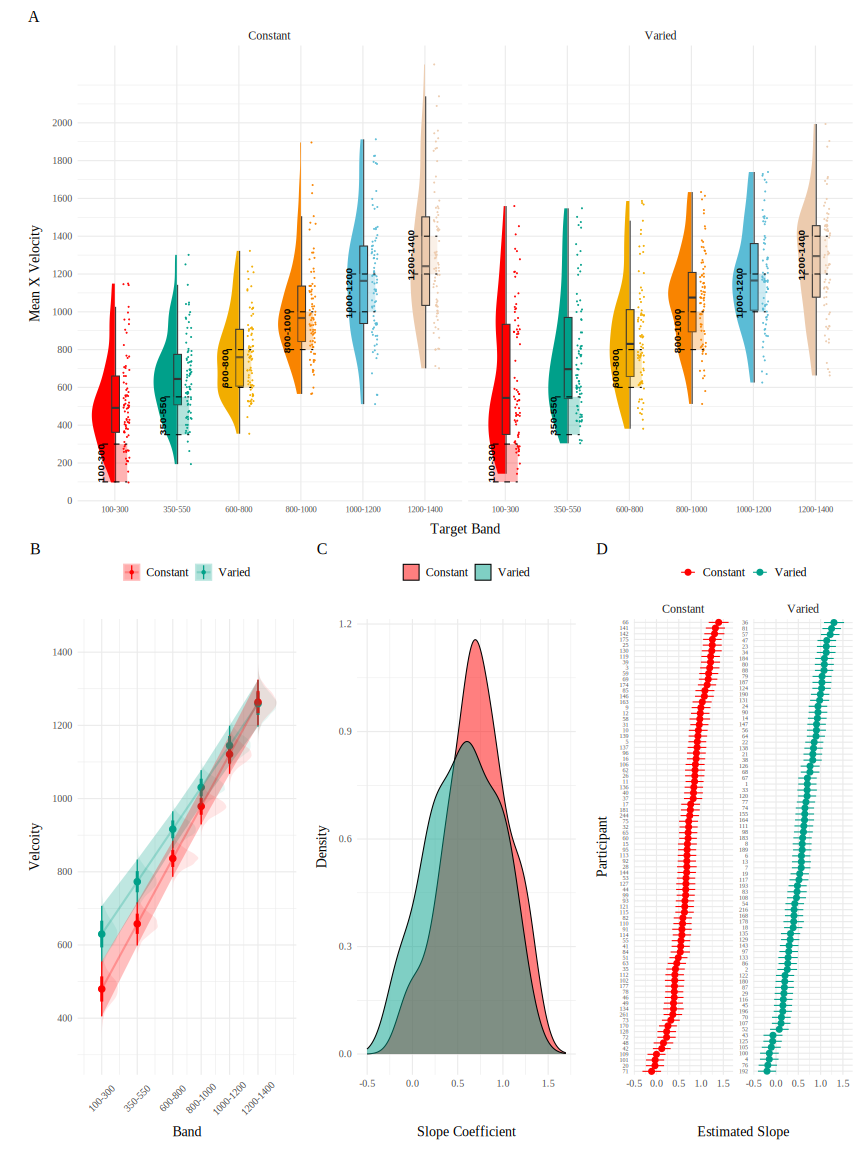
\includegraphics[width=1\textwidth,height=\textheight]{manuscript_files/figure-pdf/fig-e1-test-vx-1.pdf}

}

\caption{\label{fig-e1-test-vx}E1 testing x velocities. Translucent
bands with dash lines indicate the correct range for each velocity
band.}

\end{figure}%

\begin{table}

\caption{\label{tbl-e1-test-nf-vx}Testing vx - Empirical Summary}

\begin{minipage}[t]{\linewidth}

\begin{tabular}[t]{llrrr}
\toprule
Band & Band Type & Mean & Median & Sd\\
\midrule
100-300 & Extrapolation & 524 & 448 & 327\\
350-550 & Extrapolation & 659 & 624 & 303\\
600-800 & Extrapolation & 770 & 724 & 300\\
800-1000 & Trained & 1001 & 940 & 357\\
1000-1200 & Extrapolation & 1167 & 1104 & 430\\
\addlinespace
1200-1400 & Extrapolation & 1283 & 1225 & 483\\
\bottomrule
\end{tabular}

\end{minipage}%
\newline
\begin{minipage}[t]{\linewidth}

\begin{tabular}[t]{llrrr}
\toprule
Band & Band Type & Mean & Median & Sd\\
\midrule
100-300 & Extrapolation & 664 & 533 & 448\\
350-550 & Extrapolation & 768 & 677 & 402\\
600-800 & Extrapolation & 876 & 813 & 390\\
800-1000 & Trained & 1064 & 1029 & 370\\
1000-1200 & Trained & 1180 & 1179 & 372\\
\addlinespace
1200-1400 & Trained & 1265 & 1249 & 412\\
\bottomrule
\end{tabular}

\end{minipage}%

\end{table}%

\begin{table}

\caption{\label{tbl-e1-bmm-vx}Experiment 1. Bayesian Mixed Model
Predicting Vx as a function of condition (Constant vs.~Varied) and
Velocity Band}

\centering{

\begin{table}

\caption{\label{tab:tbl-e1-bmm-vx}Fit to all 6 bands}
\centering
\begin{tabular}[t]{lrrrr}
\toprule
Term & Estimate & 95\% CrI Lower & 95\% CrI Upper & pd\\
\midrule
Intercept & 408.55 & 327.00 & 490.61 & 1.00\\
conditVaried & 164.05 & 45.50 & 278.85 & 1.00\\
Band & 0.71 & 0.62 & 0.80 & 1.00\\
condit*Band & -0.14 & -0.26 & -0.01 & 0.98\\
\bottomrule
\end{tabular}
\end{table}

\begin{table}

\caption{\label{tab:tbl-e1-bmm-vx}Fit to 3 extrapolation bands}
\centering
\begin{tabular}[t]{lrrrr}
\toprule
Term & Estimate & 95\% CrI Lower & 95\% CrI Upper & pd\\
\midrule
Intercept & 478.47 & 404.00 & 551.45 & 1.00\\
conditVaried & 142.04 & 37.17 & 247.59 & 1.00\\
Band & 0.50 & 0.42 & 0.57 & 1.00\\
condit*Band & -0.07 & -0.17 & 0.04 & 0.89\\
\bottomrule
\end{tabular}
\end{table}

}

\end{table}%

See Table~\ref{tbl-e1-bmm-vx} for the full model results. The estimated
coefficient for training condition (\(B\) = 164.05, 95\% CrI {[}45.5,
278.85{]}) suggests that the varied group tends to produce harder throws
than the constant group, but is not in and of itself useful for
assessing discrimination. Most relevant to the issue of discrimination
is the slope on Velocity Band (\(B\) = 0.71, 95\% CrI {[}0.62, 0.8{]}).
Although the median slope does fall underneath the ideal of value of 1,
the fact that the 95\% credible interval does not contain 0 provides
strong evidence that participants exhibited some discrimination between
bands. The estimate for the interaction between slope and condition
(\(B\) = -0.14, 95\% CrI {[}-0.26, -0.01{]}), suggests that the
discrimination was somewhat modulated by training condition, with the
varied participants showing less senitivity between vands than the
constant condition. This difference is depicted visually in
Figure~\ref{fig-e1-bmm-vx}.@tbl-e1-slope-quartile shows the average
slope coefficients for varied and constant participants separately for
each quartile. The constant participant participants appear to have
larger slopes across quartiles, but the difference between conditions
may be less pronounced for the top quartiles of subjects who show the
strongest discrimination. Figure Figure~\ref{fig-e1-bmm-bx2} shows the
distributions of slope values for each participant, and the compares the
probability density of slope coefficients between training conditions.
Figure~\ref{fig-e1-indv-slopes}

The second model, which focused solely on extrapolation bands, revealed
similar patterns. The Velocity Band term (\(B\) = 0.5, 95\% CrI {[}0.42,
0.57{]}) still demonstrates a high degree of discrimination ability.
However, the posterior distribution for interaction term (\(B\) = -0.07,
95\% CrI {[}-0.17, 0.04{]} ) does across over 0, suggesting that the
evidence for decreased discrimination ability for the varied
participants is not as strong when considering only the three
extrapolation bands.

\begin{figure}

\begin{minipage}[t]{0.50\linewidth}

\centering{

\includegraphics[width=1\textwidth,height=\textheight]{manuscript_files/figure-pdf/fig-e1-bmm-vx-1.pdf}

}

\subcaption{\label{fig-e1-bmm-vx-1}Model fit to all 6 bands}

\end{minipage}%
%
\begin{minipage}[t]{0.50\linewidth}

\centering{

\includegraphics[width=1\textwidth,height=\textheight]{manuscript_files/figure-pdf/fig-e1-bmm-vx-2.pdf}

}

\subcaption{\label{fig-e1-bmm-vx-2}Model fit to only 3 extrapolation
bands}

\end{minipage}%

\caption{\label{fig-e1-bmm-vx}Conditional effect of training condition
and Band. Ribbons indicate 95\% HDI. The steepness of the lines serves
as an indicator of how well participants discriminated between velocity
bands.}

\end{figure}%

\begin{table}

\caption{\label{tbl-e1-slope-quartile}Slope coefficients by quartile,
per condition}

\centering{

\begin{tabular}[t]{l|r|r|r|r|r}
\hline
Condition & Q\_0\%\_mean & Q\_25\%\_mean & Q\_50\%\_mean & Q\_75\%\_mean & Q\_100\%\_mean\\
\hline
Constant & -0.106 & 0.478 & 0.691 & 0.929 & 1.4\\
\hline
Varied & -0.201 & 0.272 & 0.589 & 0.897 & 1.3\\
\hline
\end{tabular}

}

\end{table}%

\begin{figure}

\begin{minipage}[t]{0.50\linewidth}

\centering{

\includegraphics[width=1\textwidth,height=\textheight]{manuscript_files/figure-pdf/fig-e1-bmm-bx2-1.pdf}

}

\subcaption{\label{fig-e1-bmm-bx2-1}Slope estimates by participant -
ordered from lowest to highest within each condition.}

\end{minipage}%
%
\begin{minipage}[t]{0.50\linewidth}

\centering{

\includegraphics[width=1\textwidth,height=\textheight]{manuscript_files/figure-pdf/fig-e1-bmm-bx2-2.pdf}

}

\subcaption{\label{fig-e1-bmm-bx2-2}Destiny of slope coefficients by
training group}

\end{minipage}%

\caption{\label{fig-e1-bmm-bx2}Slope distributions between condition}

\end{figure}%

\begin{figure}

\centering{

\centering{

\includegraphics[width=1\textwidth,height=\textheight]{manuscript_files/figure-pdf/fig-e1-indv-slopes-1.pdf}

}

\subcaption{\label{fig-e1-indv-slopes-1}subset with largest slopes}

\centering{

\includegraphics[width=1\textwidth,height=\textheight]{manuscript_files/figure-pdf/fig-e1-indv-slopes-2.pdf}

}

\subcaption{\label{fig-e1-indv-slopes-2}subset with smallest slopes}

}

\caption{\label{fig-e1-indv-slopes}Subset of Varied and Constant
Participants with the smallest and largest estimated slope values. Red
lines represent the best fitting line for each participant, gray lines
are 200 random samples from the posterior distribution. Colored points
and intervals at each band represent the empirical median and 95\% HDI.}

\end{figure}%

\section{Experiment 2}\label{experiment-2}

Figure~\ref{fig-design-e2} illustrates the design of Experiment 2. The
stages of the experiment (i.e.~training, testing no-feedback, test with
feedback), are identical to that of Experiment 1. The only change is
that Experiment 2 participants train, and then test, on bands in the
reverse order of Experiment 1 (i.e.~training on the softer bands; and
testing on the harder bands).

\begin{figure*}

\centering{

\includegraphics[width=6in,height=2.5in]{manuscript_files/figure-latex/dot-figure-2.png}

}

\caption{\label{fig-design-e2}Experiment 2 Design. Constant and Varied
participants complete different training conditions. The training and
testing bands are the reverse of Experiment 1.}

\end{figure*}%

\subsection{E2 Results}\label{e2-results}

\subsubsection{Testing Phase - No
feedback.}\label{testing-phase---no-feedback.-1}

In the first part of the testing phase, participants are tested from
each of the velocity bands, and receive no feedback after each throw.

\paragraph{Deviation From Target
Band}\label{deviation-from-target-band-1}

Descriptive summaries testing deviation data are provided in
Table~\ref{tbl-e2-test-nf-deviation} and Figure~\ref{fig-e2-test-dev}.
To model differences in accuracy between groups, we used Bayesian mixed
effects regression models to the trial level data from the testing
phase. The primary model predicted the absolute deviation from the
target velocity band (dist) as a function of training condition
(condit), target velocity band (band), and their interaction, with
random intercepts and slopes for each participant (id).

\begin{equation}
dist_{ij} = \beta_0 + \beta_1 \cdot condit_{ij} + \beta_2 \cdot band_{ij} + \beta_3 \cdot condit_{ij} \cdot band_{ij} + b_{0i} + b_{1i} \cdot band_{ij} + \epsilon_{ij}
\end{equation}

\begin{table}

\caption{\label{tbl-e2-test-nf-deviation}Testing Deviation - Empirical
Summary}

\centering{

\begin{tabular}[t]{l|l|r|r|r}
\hline
Band & Band Type & Mean & Median & Sd\\
\hline
100-300 & Extrapolation & 206 & 48 & 317\\
\hline
350-550 & Extrapolation & 194 & 86 & 268\\
\hline
600-800 & Trained & 182 & 112 & 240\\
\hline
800-1000 & Extrapolation & 200 & 129 & 233\\
\hline
1000-1200 & Extrapolation & 238 & 190 & 234\\
\hline
1200-1400 & Extrapolation & 311 & 254 & 288\\
\hline
\end{tabular}

\begin{tabular}[t]{l|l|r|r|r}
\hline
Band & Band Type & Mean & Median & Sd\\
\hline
100-300 & Trained & 153 & 25 & 266\\
\hline
350-550 & Trained & 138 & 53 & 233\\
\hline
600-800 & Trained & 160 & 120 & 183\\
\hline
800-1000 & Extrapolation & 261 & 207 & 257\\
\hline
1000-1200 & Extrapolation & 305 & 258 & 273\\
\hline
1200-1400 & Extrapolation & 363 & 314 & 297\\
\hline
\end{tabular}

}

\end{table}%

\begin{figure}

\centering{

\includegraphics[width=1\textwidth,height=\textheight]{manuscript_files/figure-pdf/fig-e2-test-dev-1.pdf}

}

\caption{\label{fig-e2-test-dev}E2. Deviations from target band during
testing without feedback stage.}

\end{figure}%

\begin{table}

\caption{\label{tbl-e2-bmm-dist}Experiment 2. Bayesian Mixed Model
predicting absolute deviation as a function of condition (Constant
vs.~Varied) and Velocity Band}

\centering{

\begin{tabular}{lrrrr}
\toprule
Term & Estimate & 95\% CrI Lower & 95\% CrI Upper & pd\\
\midrule
Intercept & 151.71 & 90.51 & 215.86 & 1.00\\
conditVaried & -70.33 & -156.87 & 16.66 & 0.94\\
Band & 0.10 & 0.02 & 0.18 & 1.00\\
condit*Band & 0.12 & 0.02 & 0.23 & 0.99\\
\bottomrule
\end{tabular}

\begin{table}

\caption{\label{tab:tbl-e2-bmm-dist}Contrasts}
\centering
\begin{tabular}[t]{l|r|r|r|r|r}
\hline
contrast & Band & value & lower & upper & pd\\
\hline
Constant - Varied & 100 & 57.6 & -20.5 & 135.32 & 0.93\\
\hline
Constant - Varied & 350 & 26.6 & -30.9 & 83.84 & 0.83\\
\hline
Constant - Varied & 600 & -4.3 & -46.7 & 38.52 & 0.58\\
\hline
Constant - Varied & 800 & -29.3 & -69.4 & 11.29 & 0.92\\
\hline
Constant - Varied & 1000 & -54.6 & -101.1 & -5.32 & 0.98\\
\hline
Constant - Varied & 1200 & -79.6 & -139.5 & -15.45 & 0.99\\
\hline
\end{tabular}
\end{table}

}

\end{table}%

The model predicting absolute deviation showed a modest tendency for the
varied training group to have lower deviation compared to the constant
training group (β = -70.33, 95\% CI {[}-156.87, 16.66{]}),with 94\% of
the posterior distribution being less than 0. This suggests a potential
benefit of training with variation, though the evidence is not
definitive.

\section{Experiment 3}\label{experiment-3}

The major manipulation adjustment of experiment 3 is for participants to
receive ordinal feedback during training, in contrast to the continuous
feedback of the earlier experiments. Ordinal feedback informs
participants whether a throw was too soft, too hard, or fell within the
target velocity range. Experiment 3 participants were randomly assigned
to both a training condition (Constant vs.~Varied) and a Band Order
condition (original order used in Experiment 1, or the Reverse order of
Experiment 2).

\subsection{Results}\label{results-1}

\subsubsection{Testing Phase - No
feedback.}\label{testing-phase---no-feedback.-2}

In the first part of the testing phase, participants are tested from
each of the velocity bands, and receive no feedback after each throw.
Note that these no-feedback testing trials are identical to those of
Experiment 1 and 2, as the ordinal feedback only occurs during the
training phase, and final testing phase, of Experiment 3.

\paragraph{Deviation From Target
Band}\label{deviation-from-target-band-2}

Descriptive summaries testing deviation data are provided in
Table~\ref{tbl-e3-test-nf-deviation} and Figure~\ref{fig-e3-test-dev}.
To model differences in accuracy between groups, we fit Bayesian mixed
effects regression models to the trial level data from the testing
phase. The primary model predicted the absolute deviation from the
target velocity band (dist) as a function of training condition
(condit), target velocity band (band), and their interaction, with
random intercepts and slopes for each participant (id).

\begin{table}

\caption{\label{tbl-e3-test-nf-deviation}Testing Deviation - Empirical
Summary}

\centering{

\begin{tabular}[t]{l|l|r|r|r}
\hline
Band & Band Type & Mean & Median & Sd\\
\hline
100-300 & Extrapolation & 396 & 325 & 350\\
\hline
350-550 & Extrapolation & 278 & 176 & 299\\
\hline
600-800 & Extrapolation & 173 & 102 & 215\\
\hline
800-1000 & Trained & 225 & 126 & 284\\
\hline
1000-1200 & Extrapolation & 253 & 192 & 271\\
\hline
1200-1400 & Extrapolation & 277 & 210 & 262\\
\hline
\end{tabular}

\begin{tabular}[t]{l|l|r|r|r}
\hline
Band & Band Type & Mean & Median & Sd\\
\hline
100-300 & Extrapolation & 383 & 254 & 385\\
\hline
350-550 & Extrapolation & 287 & 154 & 318\\
\hline
600-800 & Extrapolation & 213 & 140 & 244\\
\hline
800-1000 & Trained & 199 & 142 & 209\\
\hline
1000-1200 & Trained & 222 & 163 & 221\\
\hline
1200-1400 & Trained & 281 & 227 & 246\\
\hline
\end{tabular}

\begin{tabular}[t]{l|l|r|r|r}
\hline
Band & Band Type & Mean & Median & Sd\\
\hline
100-300 & Extrapolation & 403 & 334 & 383\\
\hline
350-550 & Extrapolation & 246 & 149 & 287\\
\hline
600-800 & Trained & 155 & 82 & 209\\
\hline
800-1000 & Extrapolation & 207 & 151 & 241\\
\hline
1000-1200 & Extrapolation & 248 & 220 & 222\\
\hline
1200-1400 & Extrapolation & 322 & 281 & 264\\
\hline
\end{tabular}

\begin{tabular}[t]{l|l|r|r|r}
\hline
Band & Band Type & Mean & Median & Sd\\
\hline
100-300 & Trained & 153 & 0 & 307\\
\hline
350-550 & Trained & 147 & 55 & 258\\
\hline
600-800 & Trained & 159 & 107 & 192\\
\hline
800-1000 & Extrapolation & 221 & 160 & 235\\
\hline
1000-1200 & Extrapolation & 244 & 185 & 235\\
\hline
1200-1400 & Extrapolation & 324 & 264 & 291\\
\hline
\end{tabular}

}

\end{table}%

\begin{figure}

\centering{

\includegraphics[width=1\textwidth,height=\textheight]{manuscript_files/figure-pdf/fig-e3-test-dev-1.pdf}

}

\caption{\label{fig-e3-test-dev}e3. Deviations from target band during
testing without feedback stage.}

\end{figure}%

\begin{table}

\caption{\label{tbl-e3-bmm-dist}Experiment 3. Bayesian Mixed Model
predicting absolute deviation as a function of condition (Constant
vs.~Varied) and Velocity Band}

\centering{

\begin{tabular}{lrrrr}
\toprule
Term & Estimate & 95\% CrI Lower & 95\% CrI Upper & pd\\
\midrule
Intercept & 306.47 & 243.89 & 368.75 & 1.00\\
conditVaried & -90.65 & -182.79 & 3.75 & 0.97\\
Band & -0.07 & -0.13 & 0.00 & 0.97\\
condit*Band & 0.09 & -0.01 & 0.19 & 0.96\\
\bottomrule
\end{tabular}

}

\end{table}%

The effect of training condition in Experiment 3 showed a similar
pattern to Experiment 2, with the varied group tending to have lower
deviation than the constant group (β = -90.65, 95\% CrI {[}-182.79,
3.75{]}), with 97\% of the posterior distribution falling under 0.

\begin{figure}

\centering{

\includegraphics[width=1\textwidth,height=\textheight]{manuscript_files/figure-pdf/fig-e3-bmm-dist-1.pdf}

}

\caption{\label{fig-e3-bmm-dist}e3. Conditioinal Effect of Training
Condition and Band. Ribbon indicated 95\% Credible Intervals.}

\end{figure}%

\paragraph{Discrimination between Velocity
Bands}\label{discrimination-between-velocity-bands}

In addition to accuracy/deviation. We also assessed the ability of
participants to reliably discriminate between the velocity bands
(i.e.~responding differently when prompted for band 600-800 than when
prompted for band 150-350). Table~\ref{tbl-e3-test-nf-vx} shows
descriptive statistics of this measure, and Figure 1 visualizes the full
distributions of throws for each combination of condition and velocity
band. To quantify discrimination, we again fit Bayesian Mixed Models as
above, but this time the dependent variable was the raw x velocity
generated by participants.

\begin{equation}
vx_{ij} = \beta_0 + \beta_1 \cdot condit_{ij} + \beta_2 \cdot bandInt_{ij} + \beta_3 \cdot condit_{ij} \cdot bandInt_{ij} + b_{0i} + b_{1i} \cdot bandInt_{ij} + \epsilon_{ij}
\end{equation}

\begin{figure*}

\centering{

\includegraphics[width=1\textwidth,height=\textheight]{manuscript_files/figure-pdf/fig-e3-test-vx-1.pdf}

}

\caption{\label{fig-e3-test-vx}e3 testing x velocities. Translucent
bands with dash lines indicate the correct range for each velocity
band.}

\end{figure*}%

\begin{table}

\caption{\label{tbl-e3-test-nf-vx}Testing vx - Empirical Summary}

\centering{

\begin{tabular}[t]{l|l|r|r|r}
\hline
Band & Band Type & Mean & Median & Sd\\
\hline
100-300 & Extrapolation & 680 & 625 & 370\\
\hline
350-550 & Extrapolation & 771 & 716 & 357\\
\hline
600-800 & Extrapolation & 832 & 786 & 318\\
\hline
800-1000 & Trained & 1006 & 916 & 417\\
\hline
1000-1200 & Extrapolation & 1149 & 1105 & 441\\
\hline
1200-1400 & Extrapolation & 1180 & 1112 & 443\\
\hline
\end{tabular}

\begin{tabular}[t]{l|l|r|r|r}
\hline
Band & Band Type & Mean & Median & Sd\\
\hline
100-300 & Extrapolation & 667 & 554 & 403\\
\hline
350-550 & Extrapolation & 770 & 688 & 383\\
\hline
600-800 & Extrapolation & 869 & 814 & 358\\
\hline
800-1000 & Trained & 953 & 928 & 359\\
\hline
1000-1200 & Trained & 1072 & 1066 & 388\\
\hline
1200-1400 & Trained & 1144 & 1093 & 426\\
\hline
\end{tabular}

\begin{tabular}[t]{l|l|r|r|r}
\hline
Band & Band Type & Mean & Median & Sd\\
\hline
100-300 & Extrapolation & 684 & 634 & 406\\
\hline
350-550 & Extrapolation & 729 & 679 & 350\\
\hline
600-800 & Trained & 776 & 721 & 318\\
\hline
800-1000 & Extrapolation & 941 & 883 & 387\\
\hline
1000-1200 & Extrapolation & 1014 & 956 & 403\\
\hline
1200-1400 & Extrapolation & 1072 & 1014 & 442\\
\hline
\end{tabular}

\begin{tabular}[t]{l|l|r|r|r}
\hline
Band & Band Type & Mean & Median & Sd\\
\hline
100-300 & Trained & 392 & 270 & 343\\
\hline
350-550 & Trained & 540 & 442 & 343\\
\hline
600-800 & Trained & 642 & 588 & 315\\
\hline
800-1000 & Extrapolation & 943 & 899 & 394\\
\hline
1000-1200 & Extrapolation & 1081 & 1048 & 415\\
\hline
1200-1400 & Extrapolation & 1185 & 1129 & 500\\
\hline
\end{tabular}

}

\end{table}%

\begin{table}

\caption{\label{tbl-e3-bmm-vx}Experiment 3. Bayesian Mixed Model
Predicting Vx as a function of condition (Constant vs.~Varied) and
Velocity Band}

\centering{

\begin{tabular}{lrrrr}
\toprule
Term & Estimate & 95\% CrI Lower & 95\% CrI Upper & pd\\
\midrule
Intercept & 607.67 & 536.02 & 679.87 & 1\\
conditVaried & -167.76 & -277.14 & -64.08 & 1\\
Band & 0.44 & 0.35 & 0.52 & 1\\
condit*Band & 0.18 & 0.06 & 0.31 & 1\\
\bottomrule
\end{tabular}

}

\end{table}%

See Table~\ref{tbl-e3-bmm-vx} for the full model results.

Slope estimates for experiment 3 suggest that participants were capable
of distinguishing between velocity bands even when provided only ordinal
feedback during training (β = 0.44, 95\% CrI {[}0.35, 0.52{]}). Unlike
the previous two experiments, the posterior distribution for the
interaction between condition and band was consistently positive,
suggestive of superior discrimination for the varied participants β =
0.18, 95\% CrI {[}0.06, 0.31{]}.

\section{Modeling}\label{modeling}

In project 1, we applied model-based techniques to quantify and control
for the similarity between training and testing experience, which in
turn enabled us to account for the difference between varied and
constant training via an extended version of a similarity based
generalization model. In project 2, we will go a step further,
implementing a full process model capable of both 1) producing novel
responses and 2) modeling behavior in both the learning and testing
stages of the experiment. For this purpose, we will apply the
associative learning model (ALM) and the EXAM model of function learning
(DeLosh 1997). ALM is a simple connectionist learning model which
closely resembles Kruschke's ALCOVE model (Kruscke 1992), with
modifications to allow for the generation of continuous responses.

\subsection{ALM \& Exam Description}\label{alm-exam-description}

DeLosh et al. (\citeproc{ref-deloshExtrapolationSineQua1997}{1997})
introduced the associative learning model (ALM), a connectionist model
within the popular class of radial-basis networks. ALM was inspired by,
and closely resembles Kruschke's influential ALCOVE model of
categorization
(\citeproc{ref-kruschkeALCOVEExemplarbasedConnectionist1992}{Kruschke,
1992}).

ALM is a localist neural network model, with each input node
corresponding to a particular stimulus, and each output node
corresponding to a particular response value. The units in the input
layer activate as a function of their Gaussian similarity to the input
stimulus. So, for example, an input stimulus of value 55 would induce
maximal activation of the input unit tuned to 55. Depending on thevalue
of the generalization parameter, the nearby units (e.g.~54 and 56; 53
and 57) may also activate to some degree. ALM is structured with input
and output nodes that correspond to regions of the stimulus space, and
response space, respectively. The units in the input layer activate as a
function of their similarity to a presented stimulus. As was the case
with the exemplar-based models, similarity in ALM is exponentially
decaying function of distance. The input layer is fully connected to the
output layer, and the activation for any particular output node is
simply the weighted sum of the connection weights between that node and
the input activations. The network then produces a response by taking
the weighted average of the output units (recall that each output unit
has a value corresponding to a particular response). During training,
the network receives feedback which activates each output unit as a
function of its distance from the ideal level of activation necessary to
produce the correct response. The connection weights between input and
output units are then updated via the standard delta learning rule,
where the magnitude of weight changes are controlled by a learning rate
parameter.

See for a full specification of the equations that define ALM and EXAM.

\newpage{}

\subsection{Model Table}\label{model-table}

\subsubsection{ALM Activation \&
Response}\label{alm-activation-response}

\begin{longtable}[]{@{}
  >{\raggedright\arraybackslash}p{(\columnwidth - 4\tabcolsep) * \real{0.2069}}
  >{\raggedright\arraybackslash}p{(\columnwidth - 4\tabcolsep) * \real{0.3448}}
  >{\raggedright\arraybackslash}p{(\columnwidth - 4\tabcolsep) * \real{0.4483}}@{}}
\toprule\noalign{}
\begin{minipage}[b]{\linewidth}\raggedright
Step
\end{minipage} & \begin{minipage}[b]{\linewidth}\raggedright
Equation
\end{minipage} & \begin{minipage}[b]{\linewidth}\raggedright
Description
\end{minipage} \\
\midrule\noalign{}
\endhead
\bottomrule\noalign{}
\endlastfoot
\textbf{ALM Activation \& Response} & & \\
Input Activation &
\(a_i(X) = \frac{e^{-c(X-X_i)^2}}{\sum_{k=1}^M e^{-c(X-X_k)^2}}\) &
Activation of each input node \(X_i\), is a function of the Gaussian
similarity between the node value and stimulus X. \\
Output Activation & \(O_j(X) = \sum_{k=1}^M w_{ji} \cdot a_i(X)\) &
Activation of each Output unit \(O_j\) is the weighted sum of the input
activations and association weights. \\
Output Probability & \(P[Y_j|X] = \frac{O_j(X)}{\sum_{k=1}^M O_k(X)}\) &
Each output node has associated response, \(Y_j\). The probability of
response \(Y_j\) is determined by the ratio of output activations. \\
Mean Output &
\(m(x) = \sum_{j=1}^L Y_j \cdot \frac{O_j(x)}{\sum_{k=1}^M O_k(X)}\) &
The response to stimulus x is the weighted average of the response
probabilities. \\
\textbf{ALM Learning} & & \\
Feedback Activation & \(f_j(Z) = e^{-c(Z-Y_j)^2}\) & After responding,
feedback signal Z is presented, activating each output node via the
Gaussian similarity to the ideal response. \\
Update Weights &
\(w_{ji}(t + 1) = w_{ji}(t) + \alpha \cdot (f_j(Z(t)) - O_j(X(t)) \cdot a_i(X(t))\)
& Delta rule to update weights. Magnitude of weight changes controlled
by learning rate parameter alpha. \\
\textbf{EXAM} & & \\
Extrapolation & \(P[X_i|X] = \frac{a_i(X)}{\sum_{k=1}^M a_k(X)}\) &
Novel test stimulus X activates input nodes associated with trained
stimuli. \\
&
\(E[Y|X_i] = m(X_i) + \frac{m(X_{i+1})-m(X_{i-1})}{X_{i+1}-X_{i-1}} \cdot [X - X_i]\)
& Slope value computed from nearest training instances and then added to
the response associated with the nearest training instance,m(x) \\
\end{longtable}

\newpage{}

\subsection{Model Fitting and
Comparison}\label{model-fitting-and-comparison}

Following the procedure used by M. Mcdaniel et al.
(\citeproc{ref-mcdanielPredictingTransferPerformance2009}{2009}), we
will assess the ability of both ALM and EXAM to account for the
empirical data when fitting the models to 1) only the training data, and
2) both training and testing data. Models will be fit directly to the
trial by trial data of each individual participants, both by minimizing
the root-mean squared deviation (RMSE), and by maximizing log
likelihood. Because ALM has been shown to do poorly at accounting for
human patterns extrapolation
(\citeproc{ref-deloshExtrapolationSineQua1997}{DeLosh et al., 1997}), we
will also fit the extended EXAM version of the model, which operates
identically to ALM during training, but includes a linear extrapolation
mechanism for generating novel responses during testing.

\section*{References}\label{references}
\addcontentsline{toc}{section}{References}

\phantomsection\label{refs}
\begin{CSLReferences}{1}{0}
\bibitem[\citeproctext]{ref-bottNonmonotonicExtrapolationFunction2004}
Bott, L., \& Heit, E. (2004). Nonmonotonic {Extrapolation} in {Function
Learning}. \emph{Journal of Experimental Psychology: Learning, Memory,
and Cognition}, \emph{30}, 38--50.

\bibitem[\citeproctext]{ref-brehmerHypothesesRelationsScaled1974}
Brehmer, B. (1974). Hypotheses about relations between scaled variables
in the learning of probabilistic inference tasks. \emph{Organizational
Behavior and Human Performance}, \emph{11}(1), 1--27.
\url{https://doi.org/10.1016/0030-5073(74)90002-6}

\bibitem[\citeproctext]{ref-burknerBrmsPackageBayesian2017}
Bürkner, P.-C. (2017). Brms: {An R Package} for {Bayesian Multilevel
Models Using Stan}. \emph{Journal of Statistical Software}, \emph{80},
1--28. \url{https://doi.org/10.18637/jss.v080.i01}

\bibitem[\citeproctext]{ref-carrollFunctionalLearningLearning1963}
Carroll, J. D. (1963). Functional {Learning}: {The Learning} of
{Continuous Functional Mappings Relating Stimulus} and {Response
Continua}. \emph{ETS Research Bulletin Series}, \emph{1963}(2), i--144.
\url{https://doi.org/10.1002/j.2333-8504.1963.tb00958.x}

\bibitem[\citeproctext]{ref-deloshExtrapolationSineQua1997}
DeLosh, E. L., McDaniel, M. A., \& Busemeyer, J. R. (1997).
Extrapolation: {The Sine Qua Non} for {Abstraction} in {Function
Learning}. \emph{Journal of Experimental Psychology: Learning, Memory,
and Cognition}, 19.

\bibitem[\citeproctext]{ref-jonesActiveFunctionLearning2018}
Jones, A., Schulz, E., Meder, B., \& Ruggeri, A. (2018). \emph{Active
{Function Learning}} {[}Preprint{]}. {Animal Behavior and Cognition}.
\url{https://doi.org/10.1101/262394}

\bibitem[\citeproctext]{ref-kalishPopulationLinearExperts2004}
Kalish, M. L., Lewandowsky, S., \& Kruschke, J. K. (2004). Population of
{Linear Experts}: {Knowledge Partitioning} and {Function Learning}.
\emph{Psychological Review}, \emph{111}(4), 1072--1099.
\url{https://doi.org/10.1037/0033-295X.111.4.1072}

\bibitem[\citeproctext]{ref-kruschkeALCOVEExemplarbasedConnectionist1992}
Kruschke, J. K. (1992). {ALCOVE}: {An} exemplar-based connectionist
model of {Category Learning}. \emph{Psychological Review}, \emph{99}(1).

\bibitem[\citeproctext]{ref-makowskiBayestestRDescribingEffects2019a}
Makowski, D., Ben-Shachar, M. S., \& Lüdecke, D. (2019). {bayestestR}:
{Describing Effects} and their {Uncertainty}, {Existence} and
{Significance} within the {Bayesian Framework}. \emph{Journal of Open
Source Software}, \emph{4}(40), 1541.
\url{https://doi.org/10.21105/joss.01541}

\bibitem[\citeproctext]{ref-mcdanielConceptualBasisFunction2005}
Mcdaniel, M. A., \& Busemeyer, J. R. (2005). The conceptual basis of
function learning and extrapolation: {Comparison} of rule-based and
associative-based models. \emph{Psychonomic Bulletin \& Review},
\emph{12}(1), 24--42. \url{https://doi.org/10.3758/BF03196347}

\bibitem[\citeproctext]{ref-mcdanielPredictingTransferPerformance2009}
Mcdaniel, M., Dimperio, E., Griego, J., \& Busemeyer, J. (2009).
Predicting transfer performance: {A} comparison of competing function
learning models. \emph{Journal of Experimental Psychology. Learning,
Memory, and Cognition}, \emph{35}, 173--195.
\url{https://doi.org/10.1037/a0013982}

\bibitem[\citeproctext]{ref-rcoreteamLanguageEnvironmentStatistical2020}
Team, R. C. (2020). \emph{R: {A Language} and {Environment} for
{Statistical Computing}}. R: A Language and Environment for Statistical
Computing.

\end{CSLReferences}



\end{document}
